% !TEX root = SystemTemplate.tex
\chapter{Design  and Implementation}
The design of this project is a relativly simple one.  In order to test a program there are four steps we need to complete.
The first we need to compile the file to be tested.  Second we need to locate all the test cases for it.  Then after finding the test case we need to run the program with those test cases, and finally we need to evaluate and log the results each test case.

\begin{algorithm} [tbh]              %enter algorithm environment
\caption{Overall Algorithm}
\label{algover}
\begin{algorithmic}
	\STATE Locate all .cpp files
	\STATE Compile .cpp files
	\WHILE{Locate \_crit.tst file}
		\STATE Run \_crit.tst file
		\IF{\_crit.tst File fails}
			\IF{Any \_crit.tst fails}
				\STATE Student Fails, stop running tests
			\ENDIF
		\ENDIF
	\ENDWHILE
	\WHILE{Locate .tst file}
		\IF{Test is passed}
			\STATE $C \Leftarrow C + 1$
		\ENDIF
		\STATE $T \Leftarrow T + 1$
	\ENDWHILE
	\STATE $Percentage Passed \Leftarrow $C / T
\end{algorithmic}
\end{algorithm}
 

\section{Locate and Compile .cpp File}

\subsection{Technologies  Used}
This needed to use the dirent.h library inorder to find the .cpp file, this will be covered further in
Finding the test cases, but in general this library allows us to search for files.  Then to actually compile
the code it uses a system command to invoke g++ and compile it.

\subsection{Data Flow Diagram}
Figure~\ref{DataFlow1} Shows the Data Flow up to this point.

\begin{figure}[tbh]
\begin{center}
\includegraphics[width=0.75\textwidth]{./path}
\end{center}
\caption{Data Flow (Locate and Compile) \label{DataFlow1}}
\end{figure}


\subsection{Design Details}
Here is the code for locating the .cpp file, where root is the full path to the directory the .cpp file is located in:
\begin{lstlisting}
    DIR* dir;
    struct dirent* file;
    std::string filename;
    bool foundFlag = false;
    std::string cppFile;

    dir = opendir( root.c_str() );
    while( ( file = readdir(dir) ) != NULL && !foundFlag )
      {
        //Get the file name
        filename = file -> d_name;
        //skip over "." and ".."
        if( filename != "." && filename != ".." )
          {
        if(filename.find( ".cpp" ) != std::string::npos )
          {
            cppFile = filename;
            foundFlag = true;
          }
          }
      }


    if( !foundFlag )
      {
        std::cout << "Could not find a cpp file." << std::endl;
	std::cout << "Ending Program" << std::endl;
        return 0;
      }
\end{lstlisting}

The following is the code to compile the .cpp file, where root is the directory where the .cpp file is located
and progName is the name of the .cpp file:
\begin{lstlisting}
void Compil( std::string progName, std:: string studentName)
{
    //creat the system command and execute it.
    std::string command;
    command = "g++ " + progName + " -o " +studentName+ "_exec";
    system( command.c_str() );
}
\end{lstlisting}



\section{Locate the Test Cases }

\subsection{Technologies  Used}
This step of the program relies heavily on the dirent.h library.  It uses a recursive function to search the directory and when
it finds a subdirectory it calls itself to search that subdirectory.

\subsection{Component  Overview}
Two data types from the dirent.h library allow us to search and retrive files from directories.  The first DIR* allows us to open
a specific directory and red from it.  The second struct dirent* is the data type we use to retrive the files we read from a directory.
It has two elements that can be used to categorize the file, d\_name and d\_type.  d\_name is the name of the file, we can use this
to search for certain file extensions, and d\_type is a code for the type of file it is.  This is important in order to find which files are
subdirectories. 

\subsection{Data Flow Diagram}
Figure~\ref{DataFlow2} Shows the Data Flow up to this point.

\begin{figure}[tbh]
\begin{center}
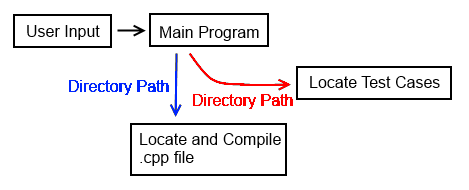
\includegraphics[width=0.75\textwidth]{./DataFlow2}
\end{center}
\caption{Data Flow (Locate and Compile) \label{DataFlow2}}
\end{figure}


\subsection{Design Details}
The following is the function to locate .tst files given a root directory:
\begin{lstlisting}
void DirCrawl( std::string rootDir, std::string &logFile , std::string exec,
        int &passed, int &tested, const std::string &masterRootDir, const std::string &studentName)
{
    struct dirent** file;	// File entry structure from dirent.h
    std::string filename;	//used in finding if a file has the extention .tst
    int n;
    n =scandir(rootDir.c_str(), &file, 0, alphasort);
    if(n == -1)
        return;

    // Read each file one at a time
    // Readdir returns next file in the directory, returns null if no other files exist
    for(int i = 2; i < n; i++)
    {
        //place file name into string filename for easier checking
        filename = std::string(file[i]->d_name);

        // checks if the file is a subdirectory, 4 is the integer idetifyer
        // for the dirent struct on Lixux systems
        if(filename != "." && filename != ".." &&  (int)file[i]->d_type == DT_DIR )
        {
            //moves into the sub-directory
            DirCrawl( rootDir + "/" + filename , logFile , exec , passed , tested,
                    masterRootDir, studentName);
        }
        else if(filename.find("_crit.tst") == std::string::npos)
        {
            // checks if the file has a .tst in it. string find returns
            // string::npos if the substring cannot be found
            if ( filename.find( ".tst") != std::string::npos )
            {
                // pass the file onto the grader 
                if (run_test_case( rootDir + "/" + filename , exec , logFile,
                            masterRootDir, studentName))
                {
                    passed += 1;
                }
                tested += 1;
            }
        }
    }
    for( int i = 0; i < n; i++)
        delete []file[i];
    delete []file;

}
\end{lstlisting}
The other parameters are passed along to functions it calls, in the case of logFile and exec and passed and tested 
keep track of the number of tests and the number of those that actually passed.


\section{Running a Test Case }

\subsection{Technologies  Used}
This part of the program is done through system calls to the linux terminal. 

\subsection{Component  Overview}
First the program to be tested is run piping the input from the .tst file and the output to a similarly named .out file.
Then using the diff command in linux the .out file, the output of the program, is compared to the .ans file, what should
have been the output of the file.  The console output is piped into a junk file which is later deleted.  If the diff command
returns zero then the files contain the same thing.

\subsection{Data Flow Diagram}
Figure~\ref{DataFlow3} Shows the Data Flow up to this point.

\begin{figure}[tbh]
\begin{center}
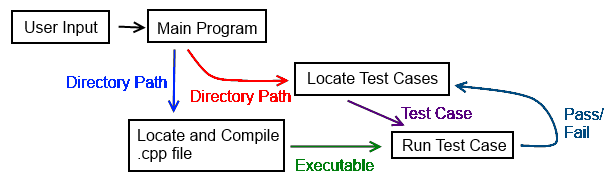
\includegraphics[width=0.75\textwidth]{./DataFlow3}
\end{center}
\caption{Data Flow (Locate and Compile) \label{DataFlow3}}
\end{figure}


\subsection{Design Details}
Here is the function to test an executable with a given test file, it gets passed the logfile to pass it to the function
that writes to the log file.  It returns true if the program passed the test case and false if it did not.
\begin{lstlisting}
bool run_test_case( std::string test_file, std::string exec,
        std::string &log_file, const std::string &rootDir, const std::string& studentName)
{
    std::string out_file = test_file;
    std::string ans_file = test_file;
    std::string test_num = "";
    std::string command_string = "";
    std::ofstream fout;
    int i=0;
    int result;
    int pos;
    int found;
    fout.open(log_file, std::ios::app | std::ios::out);
    found = test_file.find("Program_Tester_Generated_test");

    pos = test_file.find_last_of("/");

    test_num = test_file.substr( pos + 1 );
    test_num.resize(test_num.size()-4);

    if(found != std::string::npos )
    {
        found = test_file.find( "test" );
        ans_file = rootDir+"/"+ test_num;

        ans_file+=".ans";
    }
    //get text for .out file and .ans file
    //remove tst
    out_file.resize(out_file.size() - 4);
    //add out so we have case#.out
    out_file += "_" +studentName + ".out";

    //remove tst
    ans_file.resize(ans_file.size() - 3);
    //add ans so we have case#.ans
    ans_file += "ans";

    //command string = "executable < case.tst > case.out"
    //run the program with input from .tst and pipe output to .out
    command_string = exec + " < " + test_file + " > " + out_file;
    //execute the program
    std::system(command_string.c_str());

    //compare the programs output and the expected output( .out and .ans )
    // diff --ignore-all-space case.out case.ans > nul
    //if it == 0 the files were the same
    // the --ignore ignores whitespace on each line, so trailing spaces
    // or newlines aren't flagged as incorrect
    // > pipes the output into a file called nul
    command_string = "diff --ignore-all-space " + out_file + " " + ans_file+ " > nul";
    result = std::system(command_string.c_str());

    //passed test
    if ( result == 0 )
    {
        LogWrite(fout, test_num,"passed");
        fout.close();
        return true;
    }
    //failed test
    LogWrite(fout, test_num,"failed");
    fout.close();
    return false;
}

\end{lstlisting}

\section{Logging the Results}

\subsection{Technologies Used}
The fstream library is used so that we can write to a file.

\subsection{Component Overview}
There are two functions that fall into this, the first is a function that writes out the result of a single test case and the second
writes the final results of the testing.  The ofstream is opened in main to append data so that previous runs on the same
.cpp file are saved.

\subsection{Data Flow Diagram}
Figure~\ref{DataFlow4} Shows the Data Flow up to this point.

\begin{figure}[tbh]
\begin{center}
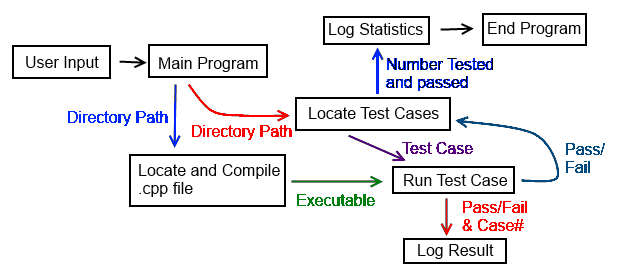
\includegraphics[width=0.75\textwidth]{./DataFlow4}
\end{center}
\caption{Data Flow (Locate and Compile) \label{DataFlow4}}
\end{figure}

\subsection{Design Details}
This first function writes the results of a single test case, it is called by the testing function after it knows determines if the case
passed.
\begin{lstlisting}
void LogWrite( std::ofstream & fout, std::string testNumber, std::string result )
{
    fout << std::left << std::setw(50)<< testNumber << std::setw(20) <<
        result.c_str() << std::endl << std::right;
}
\end{lstlisting}
The second function is called after the directory crawl returns to the main function and writes out the final result of the tests.
\begin{lstlisting}
std::string FinalLogWrite( std::string &log_file, int numPassed, int numTest )
{
    std::string tmp;
    std::ofstream fout;
    fout.open(log_file, std::ios::app | std::ios::out);
    //Calculate the number of tests failed.
    int numFailed;
    numFailed = numTest - numPassed;
    //Calculate the percent passed.
    float perPassed;
    perPassed = (float) numPassed/numTest;
    perPassed =  (int)(perPassed * 100);
    //Calculate the percent failed.
    float perFailed;
    perFailed = (float) numFailed/numTest;
    perFailed = (int)(perFailed * 100);

    //Write to stream.
    fout << "Percent of tests Passed: " << perPassed <<  "%" << std::endl;
    fout << "Percent of tests failed: " << perFailed << "%" << std::endl;
    fout.close();
    tmp = std::to_string(perPassed) + "%";
    return tmp;
}
\end{lstlisting}


